\chapter{Приложение}

В приложении мы рассмотрим пример системы, состоящей из случайного процесса с выходом в сток, функционирующим с учётом глобального условия на достижимость. Мы получим состояния этой системы на разных промежутках времени с помощью программной реализации описанного ранее вычислительного подхода и визуализируем результаты. 

Пусть задан ориентированный граф $G$, представленный на рис.\ref{fig:pic_4}:

\begin{figure}
	\centering	
	{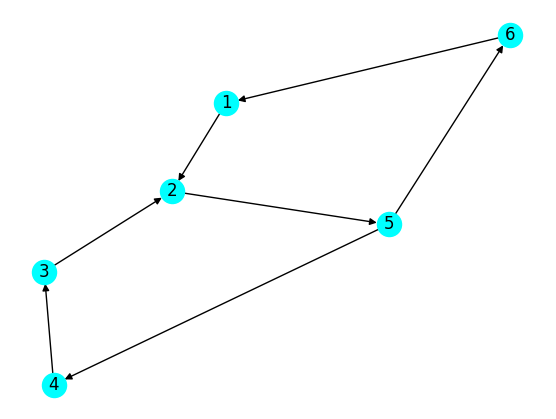
\includegraphics[width=0.9\textwidth]{img/4.png}}
	{Граф $G$}
	\label{fig:pic_4}
\end{figure}

Переходы по всем его дугам равновероятны, и таким образом он задаёт случайный процесс. Положим $k = 2$ и назначим вершину 2 выходной. Его вспомогательный граф $G'$, состоящий из двух изолированных сильно связных компонент (без стока), показан на рис.\ref{fig:pic_5}:

\begin{figure}
	\centering	
	{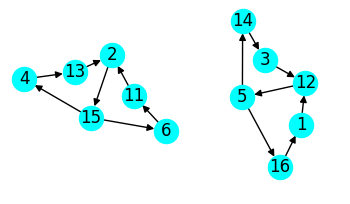
\includegraphics[width=0.9\textwidth]{img/5.png}}
	{Граф $G'$}
	\label{fig:pic_5}
\end{figure}